\documentclass{beamer}
\usetheme{Warsaw}
\usepackage[utf8]{inputenc}
\usepackage{mhchem}
\title{Présentation des tâches 3 \& 8 }
\author{Groupe 1246}
\institute{École Polytechnique de Louvain}
\date{Décembre 2014}
\begin{document}
\begin{frame}{}
\maketitle
\end{frame}

\begin{frame}{Sommaire}
\begin{itemize}
\item {Synthèse de l'ammoniac}
\item {Origine des réactifs}
\item {Empreinte écologique du procédé Haber-Bosch}
\item {Comment réduire cet impact?}
\item {Notre solution: les membranes}
\item {Conclusion}
\end{itemize}
\end{frame}

\begin{frame}{Synthèse de l'ammoniac}
$$\ce{N_{2(g)} + 3H_{2(g)} \leftrightarrows 2NH_{3(g)}}$$

\begin{itemize}
\item{Réactifs: \ce{H_2}, \ce{N_2 }}
\item{Origine $\ce{N_2} \Rightarrow$ air}
\item{Origine $\ce{H_2} \Rightarrow \cdots$}
\end{itemize}
\end{frame}

\begin{frame}{Origine de $\ce{H_2}$}
\begin{itemize}
\item{Procédé \textsc{Haber-Bosch}}
\end{itemize}

\begin{figure}[ht!]
 \centering
 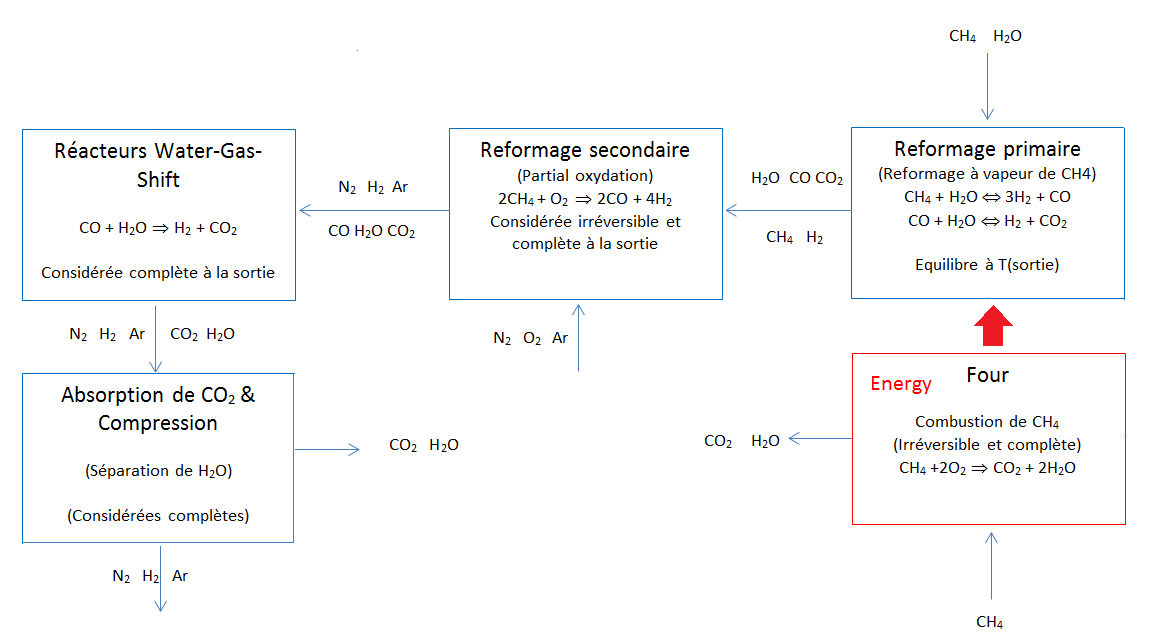
\includegraphics[scale=0.35]{PrHB2.png}
 \label{scheme}
\end{figure}
\end{frame}

\begin{frame}{\textsc{Procédé Haber-Bosch}}
	\framesubtitle{Produits du procédé}
	\begin{figure}
	\centering
	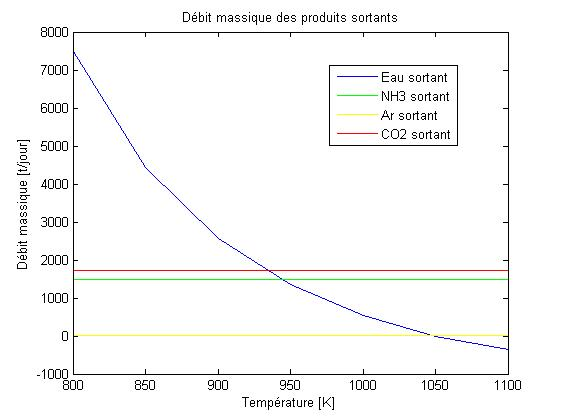
\includegraphics[scale=0.5] {produits.jpg}
	\end{figure}
\end{frame}

\begin{frame}
\frametitle{Procédé Haber-Bosh}

\framesubtitle{Provenance du \ce{CO_2} dans le procédé}
\begin{figure} [ht!]
\centering
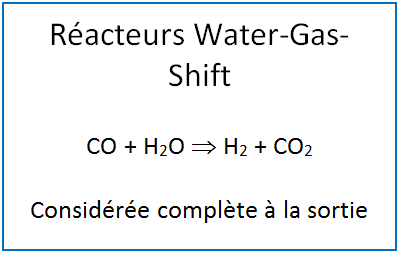
\includegraphics[scale=0.3] {Bloc_WGS.png}
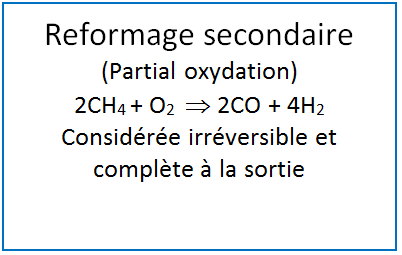
\includegraphics[scale=0.3] {Bloc_refsec.png}
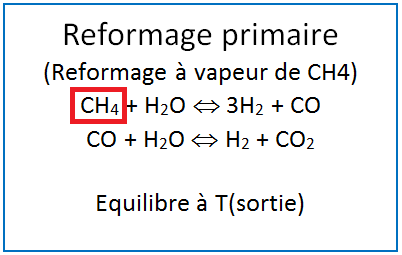
\includegraphics[scale=0.3] {Bloc_refprim.png}
\end {figure}
\end{frame}

\begin{frame}
\frametitle{Procédé Haber-Bosh}
\framesubtitle{Provenance du \ce{CO_2} dans le procédé}

Bloc de compression et absorption de \ce{CO_2}

\begin{figure} [ht!]
\centering
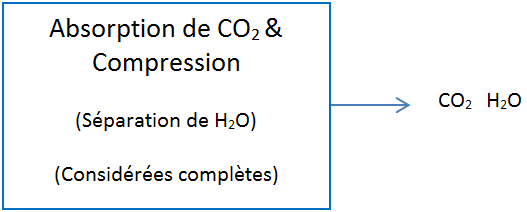
\includegraphics[scale=0.6] {Bloc_compression.png}
\end {figure}
\begin{itemize}
\item {Quantité de \ce{CO_2} rejeté : 1721 t/j }
\end{itemize}
\end{frame}



\begin{frame}{Procédé \textsc{Haber-Bosch}}
\framesubtitle{Ressources nécéssaires}

Forte utilisation d'hydrocarbures pour la production d'énergie et la réaction de vaporéformage
\begin{figure} [ht!]
\centering
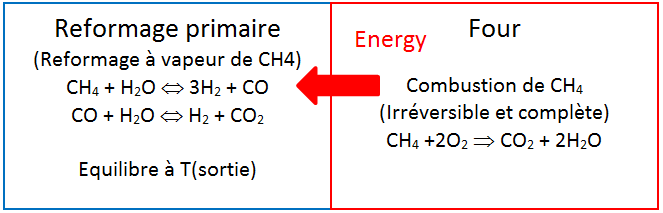
\includegraphics[scale=0.4] {energie.png}
\end{figure}
\begin{itemize}
\item {Quantité de méthane utilisée : Reformage primaire [628 t/j]  Four [63 t/j]}
\item {Rejet en \ce{CO_2} du four : 141 t/j}
\item {Quantité d'énergie nécessaire : ?}
\end{itemize}
\end{frame}

\begin{frame}{Pocédé \textsc{Haber-boch}}
\framesubtitle{Impact environnemental: résumé}
\end{frame}


\begin{frame}{Comment réduire cet impact?}
\begin{itemize}
\item {Modification du combustible du four}
\item {Meilleure isolation du four}
\item {Traitement du $\ce{CO_2}$}
\item {Modification de l'origine du $\ce{H_2}$}
\item {Installation d'une membrane au sein du réacteur de reformage primaire}
\end{itemize}
\end{frame}

\begin{frame}{Notre solution: installation d'une membrane}
\textbf{But:} réduire les émissions de \ce{CO_2}. \\
\textbf{Principe:} déplacer l'équilibre de la réaction grâce à la loi de \textsc{le-Chatelier}.
\\\textbf{Comment:} installation de membrane laissant passer l'\ce{H_2} par conduction protonique et ainsi déplacer l'équillibre vers la droite.
$$\ce{CH_4} + \ce{H_2O} \leftrightarrows 3\ce{H_2}+\ce{CO}$$
$$\ce{CO}+\ce{H_2O} \leftrightarrows \ce{CO_2}+\ce{H_2}$$
\end{frame}

\begin{frame}{Notre solution: installation d'une membrane}
\framesubtitle{Conduction protonique}
\begin{figure}[ht!]
 \centering
 \includegraphics[scale=0.25]{schemen.PNG}
 \caption{conduction protonique\footnote{https://tel.archives-ouvertes.fr/tel-00425050/document consulté le 15/12/2014} (perovskite)}
\end{figure}
\textbf{Effet:} après oxydation, transfert des protons (ions \ce{H^+}) et des \ce{e^-}, suivi d'une recomposition de l'\ce{H_2}.
\end{frame}

\begin{frame}{Notre solution: installation d'une membrane}
\framesubtitle{Effets possibles de la membrane sur le système}
\begin{itemize}
\item Réduit le besoin de catalyseur en gardant la température et le taux de conversion de \ce{CH_4} constant.
\item Augmente le taux de conversion en gardant la température et la quantité catalyseur constante.
\item Diminue le besoin en chaleur en gardant le taux de conversion et la quantité de catalyseurs constante : Le plus utile selon nous.
\end{itemize}
\end{frame}

\begin{frame}{Notre solution: installation d'une membrane}
\framesubtitle{Effet de la membrane sur la température}
\begin{itemize}
\item Pourquoi un four dans le procédé \textsc{Haber-Bocsh}? Afin déplacer l'équilibre et favoriser la réaction de conversion du \ce{CH_4} en \ce{H_2}.
\item La réaction pourra s'opérer à plus basse température
\end{itemize}

\end{frame}

\begin{frame}{Inconvénients de la méthode}
\begin{itemize}
\item Prix du aux matières constituant la membrane 
\item L'éfficacité des tubes diminue en présence de \ce{CO}
\item Ce n'est que des études, pas encore disponible de manière industrielle.
\item Consommation importante d'eau à basse température
\end{itemize}
\end{frame}

\begin{frame}{Avantages de la méthode (dépend du type de membranes)}
\begin{itemize}
\item Moins besoin du four : 
    \begin{itemize}
    \item plus d'émissions de \ce{CO_2} dû à la combustion de méthane
    \item diminue la consommation de \ce{CH_4}
    \end{itemize} 
\item Fléxibilité du point d'action de la méthode. 
\item Efficace même à base temperature
\begin{figure}[ht!]
 \centering
 \includegraphics[scale=0.25]{pressure.PNG}
 \caption{taux de conversion du méthane en fonction de la pression \footnote{http://doc.utwente.nl/50860/1/thesis_Patil.pdf
, consulté le 15/12/1994}}
\end{figure}
\end{itemize}
\end{frame}
\end{document}